\documentclass[dutch]{ucll-slides}
\usepackage{pxfonts}
\usepackage{tikz}
\usepackage{calc}
\usepackage{ucll-code}


\usetikzlibrary{calc,shadows,tikzmark}

\coursename{Scripttalen}
\title{Truthy/Falsey Waarden}

\newcommand{\nonterminal}[1]{{\color{red} \ensuremath{\langle}#1\ensuremath{\rangle}}}

\newenvironment{matchexamples}{
  \begin{center}
  \newcommand{\sep}{\hspace{5mm}}
  \newcommand{\match}[1]{\sep{\color{green!50!black} "##1"}}
  \newcommand{\mismatch}[1]{\sep{\color{red} "##1"}}
}{\end{center}}


\begin{document}

\maketitle

\section{De Java Situatie}

\frame{\tableofcontents[currentsection]}

\begin{frame}
  \frametitle{Booleaanse Waarden}
  \begin{center}
    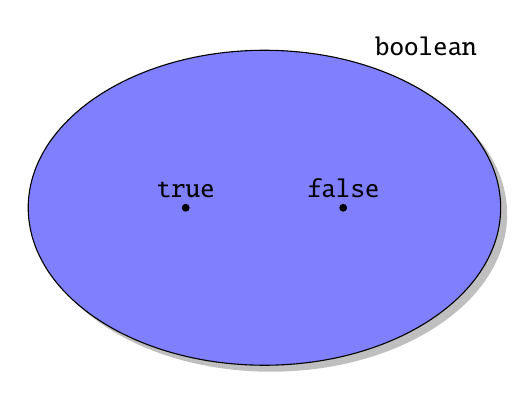
\begin{tikzpicture}
      \draw[drop shadow,fill=blue!50] (0,0) ellipse [x radius=3cm,y radius=2cm];
      \node at (45:2.9) {\ttfamily boolean};

      \path[fill=black] (-1,0) circle [radius=0.05cm] node[above] {\ttfamily true};
      \path[fill=black] (1,0) circle [radius=0.05cm] node[above] {\ttfamily false};
    \end{tikzpicture}
  \end{center}
  \begin{itemize}
    \item Er bestaat 2 \texttt{boolean}-waarden: \texttt{true} en \texttt{false}
  \end{itemize}
\end{frame}

\begin{frame}
  \frametitle{Gebruik \texttt{boolean}s}
  \code[language=java]{code.java}
  \codeunderline{java if left}{java if right}
  \codeunderline{java while left}{java while right}
  \codeunderline{java for left}{java for right}
  \codeunderline{java and op1 left}{java and op1 right}
  \codeunderline{java and op2 left}{java and op2 right}
  \codeunderline{java or op1 left}{java or op1 right}
  \codeunderline{java or op2 left}{java or op2 right}
  \codeunderline{java not left}{java not right}
  \begin{itemize}
    \item Deze statements/operators verwachten \texttt{boolean}s
    \item \texttt{if (5)} wordt door compiler verworpen
  \end{itemize}
\end{frame}


\section{De Python Situatie}

\frame{\tableofcontents[currentsection]}

\begin{frame}
  \frametitle{Booleaanse Waarden}
  \begin{center}
    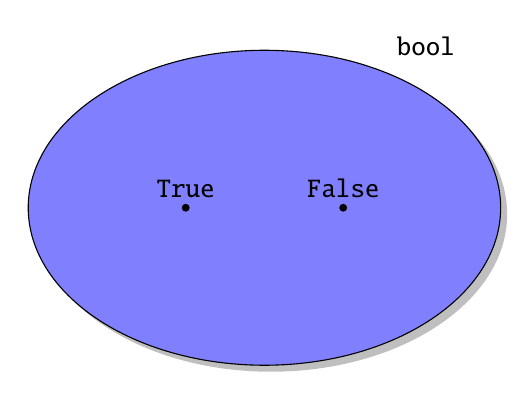
\begin{tikzpicture}
      \draw[drop shadow,fill=blue!50] (0,0) ellipse [x radius=3cm,y radius=2cm];
      \node at (45:2.9) {\ttfamily bool};

      \path[fill=black] (-1,0) circle [radius=0.05cm] node[above] {\ttfamily True};
      \path[fill=black] (1,0) circle [radius=0.05cm] node[above] {\ttfamily False};
    \end{tikzpicture}
  \end{center}
  \begin{itemize}
    \item Er bestaat 2 \texttt{bool}-waarden: \texttt{True} en \texttt{False}
    \item Let op de hoofdletters!
  \end{itemize}
\end{frame}

\begin{frame}
  \frametitle{Gebruik \texttt{bool}s}
  \code[language=python]{code.py}
  \codeunderline{python if left}{python if right}
  \codeunderline{python while left}{python while right}
  \codeunderline{python and op1 left}{python and op1 right}
  \codeunderline{python and op2 left}{python and op2 right}
  \codeunderline{python or op1 left}{python or op1 right}
  \codeunderline{python or op2 left}{python or op2 right}
  \codeunderline{python not left}{python not right}
  \begin{itemize}
    \item \texttt{True} en \texttt{False} hebben hun standaardbetekenis
    \item Wat met andere waarden? (getallen, strings, lijsten, \dots)
  \end{itemize}
\end{frame}

\begin{frame}
  \frametitle{Wat Met Niet-\texttt{bool} waarden?}
  \structure{Mogelijke Aanpak \#1}
  \begin{itemize}
    \item Zoals Java: enkel \texttt{True} en \texttt{False} toelaten
    \item Andere waarden: exceptions
  \end{itemize}
  \vskip5mm
  \structure{Mogelijke Aanpak \#2}
  \begin{itemize}
    \item W\'el andere waarden dan \texttt{True} en \texttt{False} toelaten
    \item Wat is dan de betekenis van \texttt{if 5}?
    \visible<2->{
      \item Dit is de aanpak waar Python voor koos
    }
  \end{itemize}
\end{frame}

\begin{frame}
  \frametitle{Truthy en Falsey Waarden}
  \begin{itemize}
    \item Python verdeelt wereld op in truthy en falsey waarden
  \end{itemize}
  \begin{center}
    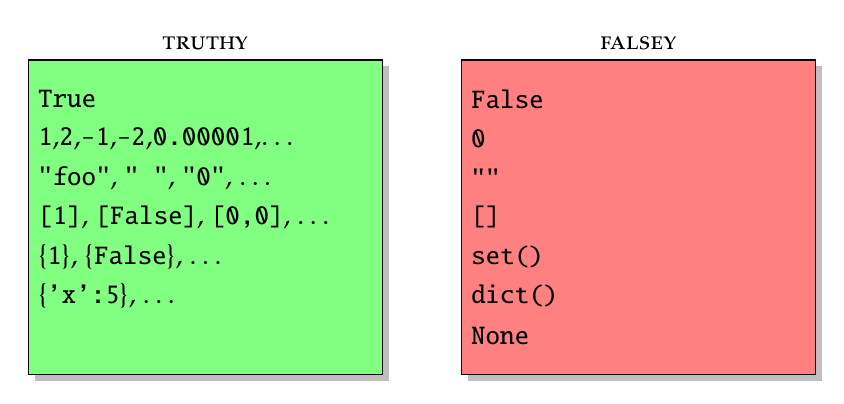
\begin{tikzpicture}
      \draw[fill=green!50,drop shadow] (-5,-2) rectangle (-0.5,2);
      \draw[fill=red!50,drop shadow] (0.5,-2) rectangle (5,2);
      \node[anchor=south] at (-2.75,2) {\scshape truthy};
      \node[anchor=south] at (2.75,2) {\scshape falsey};

      \visible<2->{
        \node[anchor=west] at (-5,1.5) {\texttt{True}};
        \node[anchor=west] at (0.5,1.5) {\texttt{False}};
      }
      \visible<3->{
        \node[anchor=west] at (-5,1) {\texttt{1},\texttt{2},\texttt{-1},\texttt{-2},\texttt{0.00001},\dots};
        \node[anchor=west] at (0.5,1) {\texttt{0}};
      }
      \visible<4->{
        \node[anchor=west] at (-5,0.5) {\texttt{"foo"}, \texttt{" "}, \texttt{"0"}, \dots};
        \node[anchor=west] at (0.5,0.5) {\texttt{""}};
      }
      \visible<5->{
        \node[anchor=west] at (-5,0) {\texttt{[1]}, \texttt{[False]}, \texttt{[0,0]}, \dots};
        \node[anchor=west] at (0.5,0) {\texttt{[]}};
      }
      \visible<6->{
        \node[anchor=west] at (-5,-0.5) {\texttt{\{1\}}, \texttt{\{False\}}, \dots};
        \node[anchor=west] at (0.5,-0.5) {\texttt{set()}};
      }
      \visible<7->{
        \node[anchor=west] at (-5,-1.0) {\texttt{\{'x':5\}}, \dots};
        \node[anchor=west] at (0.5,-1.0) {\texttt{dict()}};
      }
      \visible<8->{
        \node[anchor=west] at (0.5,-1.5) {\texttt{None}};
      }
    \end{tikzpicture}
  \end{center}
  \begin{overprint}
    \onslide<2>
    \begin{center}
      \texttt{True} is truthy, \texttt{False} is falsey
    \end{center}
    \onslide<3>
    \begin{center}
      Getallen: \texttt{0} is falsey, alle andere getallen zijn truthy
    \end{center}
    \onslide<4>
    \begin{center}
      Strings: lege string is falsey, niet-lege strings zijn truthy
    \end{center}
    \onslide<5>
    \begin{center}
      Lijsten: lege lijst is falsey, niet-lege lijsten zijn truthy
    \end{center}
    \onslide<6>
    \begin{center}
      Analoog voor sets\dots
    \end{center}
    \onslide<7>
    \begin{center}
      Analoog voor dictionaries\dots
    \end{center}
    \onslide<8>
    \begin{center}
      \texttt{None} is falsey
    \end{center}
  \end{overprint}
\end{frame}

\begin{frame}
  \frametitle{Voorbeelden}
  \begin{overprint}
    \onslide<1>
    \code[language=python]{countdown1.py}
    \onslide<2>
    \code[language=python]{queue1.py}
  \end{overprint}
  \begin{center}
    kan worden geschreven als
  \end{center}
  \vskip2mm
  \begin{overprint}
    \onslide<1>
    \code[language=python]{countdown2.py}
    \onslide<2>
    \code[language=python]{queue2.py}
  \end{overprint}
\end{frame}

\begin{frame}
  \frametitle{Stijlkeuze}
  \begin{itemize}
    \item Kies zelf welk je het meest leesbaar vindt
    \item Veel code/documentatie maakt gebruikt van truthy/falsey
    \item Let op met \texttt{== True} en \texttt{== False}
  \end{itemize}
\end{frame}

\end{document}



%%% Local Variables: 
%%% mode: latex
%%% TeX-master: t
%%% End: 
